\chapter{}

\begin{figure}
\centering
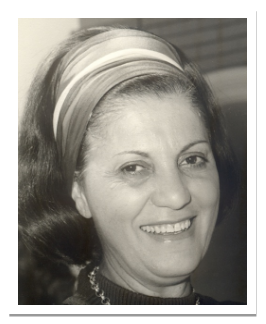
\includegraphics[width=0.7\linewidth]{13/mamãe.png}
\caption{Mamãe, por volta dos cinquenta anos.}
\end{figure}

Minha mãe tinha ideias muito claras sobre o que deveria ser uma preparação eficiente para uma vida de mulher bem sucedida.
Aprendidas ao longo da sua experiência de menina pobre e prudentemente ajustadas aos valores predominantes em nosso meio.
O modelo se desenhava a partir de três orientações básicas: ter ótima aparência, ser uma impecável dona-de-casa e estudar o suficiente para garantir desembaraço social e uma pequena, mas honrosa margem de independência financeira.
O bastante ``para os alfinetes'', para usar uma expressão de época.
O objetivo final do programa, como não podia deixar de ser, era chegar a um casamento assentado sobre uma desejável e sólida base material e afetiva.
Nessa ordem.
A novidade, em relação a tempos anteriores, é que as mulheres do pós-guerra começavam a ter ambições de um tratamento mais igualitário face aos homens.
Tomando cuidado, porém, para não perder as vantagens inerentes à decantada fragilidade do sexo.
Assim, ensinou-me ela que nascer bonita não era essencial, mesmo porque nem todas têm essa sorte, mas, com jeito, simpatia e bom gosto, pode-se parecer bonita e isso, afinal, é o que importa.
Dominar as competências domésticas era imprescindível, mas apenas para saber orientar e governar as empregadas, pois, mesmo sendo de origem humilde, minha mãe acompanhava a crença generalizada de que o trabalho doméstico era degradante.
Embora Hollywood divulgasse a visão encantadora da dona de casa de aventalzinho, feliz na sua cozinha planejada, entre seus eletrodomésticos de última geração, as brasileiras preferiam agradecer a Deus a felicidade de terem nascido numa terra onde não havia nada disso, mas a criadagem era farta e barata.
Quanto a adquirir uma profissão, o aconselhável era escolher uma atividade “mais feminina” como o magistério, por exemplo, que pela afinidade evidente com os deveres de uma mãe de família, preenchia o quesito de prover a mulher de um dinheirinho extra para os seus supérfluos, sem comprometer o cumprimento das suas obrigações prioritárias com o lar, o marido e os filhos.
O esforço intelectual exagerado também não era recomendável.
Mamãe dizia que homem nenhum quer mulher metida a sabichona.
Concedia-se, a título de consolo, que as muito feias ou desajustadas que não conseguissem casar, buscassem com mais afinco realizar-se numa profissão.
Mas, se ousassem se destacar além da conta, sobretudo nos estudos, passariam fatalmente à condição de “esquisitas”.
Muita leitura, muito estudo acabam amolecendo os miolos, era outro dos axiomas que mamãe assimilara do ambiente e gostava de recitar.

Ocorreu, porém, no meu caso, que os belos planos da minha mãe foram frustrados por dois fatores: dos nove aos dezoito anos eu não consegui permanecer magra por mais do que uns poucos meses, o que reduziu em muito minhas possibilidades no mercado casamenteiro e, a partir de certo momento, eu decidi eleger Tia Maria Angelina, a irmã caçula dela, em meu modelo predileto de desenvolvimento pessoal.


Olhando minha adolescência em retrospectiva, é possível entender de que maneira esses fatores se interligaram de modo a formar uma barreira muito sólida atrás da qual me pus a salvo de um destino que inconscientemente eu rejeitava.
Tia Maria Angelina parecia aos meus olhos de menina o suprassumo da modernidade: era bonita, alta, de uma elegância sóbria, casual, personalíssima.
Tocava violão, cantava, tinha um monte de amigos e amigas e parecia levar uma vida bem mais divertida que a das outras mulheres que eu conhecia.
Vez ou outra me levava com ela no seu \textit{Studebaker} azul, outra ousadia, um carrão que ela guiava desafiadoramente pela cidade.
E, incrível, sua irresistível vocação para sacudir aquele mundinho provinciano levou-a a abandonar um noivo praticamente ao pé do altar, ato justificado perante toda a família com o mais cândido argumento:
{\small\itshape``-- Perdão, mas eu não consigo me ver como dona-de-casa pelo resto dos meus dias, fazendo comidinha, cuidando do maridinho e dos filhinhos.
Sinto muito!''}

Eu não podia avaliar, então, o tamanho da comoção causada por esse gesto.
Mas, acho que de algum modo ela compreendeu que encerrara suas possibilidades de permanecer na cidade.
Em pouco tempo mudou-se para São Paulo, levando com ela Vô João e Vó Didi.

\begin{figure}
\centering
\includegraphics[width=0.7\linewidth]{13/manina+lygia+glória.png}
\caption{Manina e suas amigas, Lygia e Góia (Maria da Glória).}
\end{figure}

Eu resistia o quanto podia ao projeto que mamãe reservara para o meu futuro.
Tive que estudar piano com um professor que eu odiava tanto quanto ao instrumento.
Acho que se me fosse dado escolher, preferia dançar a tocar.
Mas não fui consultada.
Minha primeira apresentação em público foi um fiasco.
Esqueci a música tão longamente ensaiada.


Minha obesidade e minhas pernas tortas receberam um tratamento que incluía ginástica, natação, regimes sucessivos com sucessivos médicos e uns malditos sapatos ortopédicos que, além de divertir muito meu irmão, só resultaram em duas torturantes unhas encravadas e um andar de quem tinha urgência de ir ao banheiro.
Definitivamente, eu estava longe de ser a beldade que a minha mãe sonhava fazer debutar no Clube Araraquarense.

Ah, e havia o nariz: eu herdara do meu pai um nariz de batata que no rosto dele reforçava certa rusticidade máscula, mas em mim, eu sabia, exercia um efeito devastador.
Mesmo que Tia Maria Angelina me assegurasse que meus olhos e minha boca eram lindos, eu não me convencia de que uma coisa compensasse a outra.

A contenda entre mim e minha mãe estendeu-se por toda a minha adolescência e assumiu, em alguns momentos, proporções bastante dramáticas.
Mamãe não se conformava com minha aparência e minhas raras incursões sociais lhe davam total razão.
Refugiei-me mais e mais nos livros e iniciei um movimento de resistência passiva que sugeria o mais completo conformismo e levava minha pobre mãe à exasperação.
Comecei, secretamente, a traçar para mim um caminho que nada tinha a ver com as preocupações das outras garotas da minha idade.
Uma vez que eu não me ajustava aos padrões, optei por cultivar as diferenças e buscar uma individualidade própria que se estabeleceria a partir de uma decisão central: a de jamais me casar e escolher uma profissão que me desse, além de realização pessoal, total independência econômica.
O primeiro e essencial passo nessa direção era ir embora da cidade.
De mansinho, aos poucos, fui conquistando o conceito de ``sensata e amadurecida'' que me conferiu certa liberdade de ação e inibiu um pouco as investidas maternas.
Ia sempre que possível para São Paulo, nas férias e, com Tia Maria Angelina, sempre ela, comecei a aprender a me vestir, pentear e comportar-me de um jeito menos provinciano.
Comecei a desenhar minhas próprias roupas.

\begin{figure}
\centering
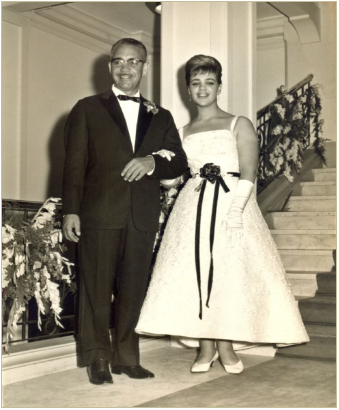
\includegraphics[width=0.7\linewidth]{13/debutando.png}
\caption{Debutando no Araraquarense.}
\end{figure}

Nem tudo eram flores, porém.
As festinhas de colégio continuavam a ser uma provação que me exigia elevada dose de estoicismo e teatral indiferença frente às minhas coleguinhas que exibiam seus corpinhos de ninfas em acrobáticos passos de \textit{rock n' roll} e \textit{hully-gully}.
Claro que a nenhum garoto ocorria convidar-me para uma empreitada dessa natureza.
Daí que, vagando ao largo das pistas de dança, acabei descobrindo pelos cantos, entre as vítimas do chamado ``chá-de-cadeira'', gente surpreendentemente interessante.
Um dia, essa descoberta se transformaria na certeza de que numa cidade tradicional e conservadora como a minha, é exatamente à margem que você vai encontrar as melhores figuras.
Também devo a essa fase outro importante aprendizado: meninos eram capazes de engrenar boas conversas quando, fora de um contexto de sedução, permitiam-se expor à vontade seus medos e inseguranças.
E, principalmente, suas opiniões e visões sobre o comportamento das garotas.
Essa iniciação no universo masculino foi especialmente útil no sentido de reforçar minha decisão de rejeitar firmemente o modelo feminino em voga, além de me despertar para o fato de que os rapazes eram, de longe, interlocutores bem mais estimulantes do que as moças.


Aos dezessete anos, terminado o Colegial, consegui meu primeiro grande triunfo: meus pais aceitaram que eu fizesse faculdade na Capital.
Confiando nos elogios que as minhas redações escolares sempre mereceram e acreditando nos efeitos do trabalho em que vinha me aplicando, ou seja, a construção da minha persona, escolhi fazer Jornalismo.
Mas a vitória tinha um preço: minha mãe queria me ver estudando no ``Sedes Sapientiae'', faculdade agregada à Pontifícia Universidade Católica de São Paulo, conhecida por abrigar algumas dezenas de herdeiras das mais antigas famílias da sociedade paulistana.
Tal sonho começara a ser alimentado muitos anos antes, quando um extravagante italiano mudou-se para a minha cidade e, após construir um casarão de estilo florentino uma esquina abaixo da minha casa, lá acomodou-se com a mulher e uma filha que só aparecia nas férias.
Quando essa filha linda, suave e elegante, numa das suas habituais passagens por sob a nossa janela, contou a Dona Lectícia que cursava a ``Sedes Sapientiae'', não houve mais quem tirasse da cabeça da mamãe que aquelas adoráveis maneiras se deviam à educação ministrada pelas Cônegas Agostinianas, dirigentes e proprietárias do tal estabelecimento.
Portanto, eu poderia fazer Jornalismo, se quisesse, mas teria que ser como opção secundária.
Porque do ``Sedes Sapientiae'' ela não arredava pé.
Concordei em candidatar-me lá ao curso de História.
Afinal, imaginei, cultura geral não seria demais para uma futura jornalista.

Ainda uma vez fui levada a um endocrinologista, o último e o mais sensato e ele me garantiu que, longe das pressões familiares, a embriaguez da liberdade certamente superaria os encantos da comida.
Preparei-me para deixar o casulo.
Poucos meses antes de embarcar, comecei a emagrecer.
Até arrumei um namorado.
Lindo.
Mas com uma voz ridícula, em falsete.
Livrei-me dele sem piedade.
Tinha coisas mais importantes em que pensar.
